\begin{frame}
  \frametitle{Задача <<Рыцарский щит>>}
  \begin{center}
    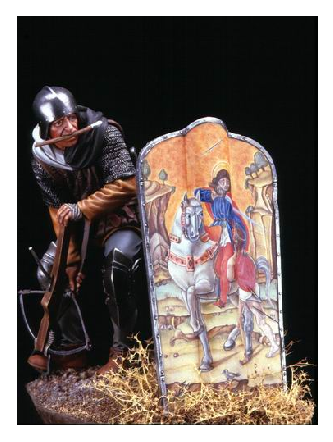
\includegraphics[height=9cm]{shield-11.eps}
  \end{center}
\end{frame}

\begin{frame}
  \frametitle{Над задачей работали}
  \begin{itemize}
    \item Идея задачи: Владимир Ульянцев
    \item Текст условия: Андрей Комаров
    \item Тесты, проверяющая программа и др.: Алексей Цыпленков
    \item Решения: Владимир Ульянцев, Нияз Нигматуллин
    \item Текст разбора: Алексей Цыпленков
  \end{itemize}
\end{frame}

\begin{frame}
  \frametitle{Формулировка задачи}
  \begin{itemize}
    \item
      Дано два треугольника
    \item
      Нужно приложить их друг к другу так, чтобы периметр получившейся фигуры был минимальным
  \end{itemize}
\end{frame}

\begin{frame}
  \frametitle{Идея решения}
  \begin{itemize}
    \item Периметр полученной фигуры "--- сумма периметров треугольников минус удвоенная длина общей части
    \item Нужно максимизировать длину общей части
  \end{itemize}
\end{frame}
              
\begin{frame}
  \frametitle{Как это сделать?}
  \begin{itemize}
    \item
      Нужно прикладывать треугольники наибольшими сторонами
    \item
			Тогда ответ равен $P_1 + P_2 - 2\min(\max(a_1, b_1, c_1), \ \max(a_2, b_2, c_2)) $
  \end{itemize}
\end{frame}

\begin{frame}
  \frametitle{Итого}
  Вопросы?
\end{frame}
